% Use the following line _only_ if you're still using LaTeX 2.09.
%\documentstyle[icml2011,epsf,natbib]{article}
% If you rely on Latex2e packages, like most moden people use this:
\documentclass{article}

% For figures
\usepackage{graphicx} % more modern
%\usepackage{epsfig} % less modern
\usepackage{subfigure} 

% For citations
\usepackage{natbib}

% For algorithms
\usepackage{algorithm}
\usepackage{algorithmic}

% As of 2010, we use the hyperref package to produce hyperlinks in the
% resulting PDF.  If this breaks your system, please commend out the
% following usepackage line and replace \usepackage{icml2011} with
% \usepackage[nohyperref]{icml2011} above.
\usepackage{hyperref}

% Packages hyperref and algorithmic misbehave sometimes.  We can fix
% this with the following command.
\newcommand{\theHalgorithm}{\arabic{algorithm}}

% Employ the following version of the ``usepackage'' statement for
% submitting the draft version of the paper for review.  This will set
% the note in the first column to ``Under review.  Do not distribute.''
\usepackage[accepted]{icml2011} 
% Employ this version of the ``usepackage'' statement after the paper has
% been accepted, when creating the final version.  This will set the
% note in the first column to ``Appearing in''
% \usepackage[accepted]{icml2011}


% The \icmltitle you define below is probably too long as a header.
% Therefore, a short form for the running title is supplied here:
\icmltitlerunning{Context Aware Movie Recommender Systems}

\begin{document} 

\twocolumn[
\icmltitle{CAMR - A Context Aware Movie Recommender System}

% It is OKAY to include author information, even for blind
% submissions: the style file will automatically remove it for you
% unless you've provided the [accepted] option to the icml2011
% package.
\icmlauthor{Primal Pappachan}{primal1@umbc.edu}
 %\icmladdress{Your Fantastic Institute,
%            314159 Pi St., Palo Alto, CA 94306 USA}
\icmlauthor{Arnav Joshi}{arnavj1@umbc.edu}
%\icmladdress{Their Fantastic Institute,
%            27182 Exp St., Toronto, ON M6H 2T1 CANADA}

% You may provide any keywords that you 
% find helpful for describing your paper; these are used to populate 
% the "keywords" metadata in the PDF but will not be shown in the document
\icmlkeywords{recommender systems, machine learning}

\vskip 0.3in
]

\section{Introduction}
The task of recommender systems is to turn data of users and their preferences into predictions of possible future likes and interests \cite{adomavicius2011context}.  The majority of existing approaches to recommender systems focuses on recommending the most relevant items to individual users. However, they do not take into consideration any contextual information, such as time, place and the company of other people (in use cases such as movies). In other words, traditional recommender systems deal with applications having only two types of entities, users and items, and do not put them into a context when providing recommendations. 
Context information is any information about the situation, circumstances and user state when a user is consuming the content item. Context can be the time of day, weather, social situation, user’s mood etc.\cite{segaran2008programming} However, the relationship between context and user decision making is very complex and difficult to model. 
Context-aware recommender systems help users and their desired content in a reasonable time, by exploiting the pieces of information that describe the situation in which users will consume the items. CAMRS models this approach by providing the recommendation on the basis of a function of user, item, previous ratings, as well as the context information provided by the user.

\subsection{Importance of context} 
The inclusion of the contextual information into the recommendation process presents opportunities for richer and more diverse interactions between the end-users and recommender systems. With the help of user's context, CAMRS will not only incorporate the user's profile of previous movies he has watched, but also include domain-dependent context modeling, which will help give better recommendation on the selection of movies.  Adapting the item choice based on the user's context can help recommend movies that might be given better ratings by the user.

\subsection{Collaborative Filtering}
Collaborative filtering systems gather item ratings as a form of user feedback for items in a given domain and exploit similarities and differences among profiles of several users in determining how to recommend an item. In movie recommendation, users provide ratings for the movies they have watched. 
A rating function in a recommendation system is one which tries to estimate the rating for the new item (here, the movie choice) based on the user's profile i.e. previous preferences.
This is done by initially generating a two-dimensional User x Item recommender matrix which takes partial user preference data as its input and produces a list of recommendations for each user as an output.
After the recommendation function is defined (or constructed) based on the available data, recommendation list for any given user u is typically generated by using the recommendation function on user u and all candidate items to obtain a predicted rating for each of the items and then by ranking all items according to their predicted rating value.
In CAMRS we hope to gain additional insight on user preferences by taking contextual information into consideration as explicit categories of data, such as the time, location and social situation(with a companion or not). The rating function r can thus be defined as: 
\begin{equation}r: User * Item * Context = Rating 
\end{equation}
The recommendation will be on a Likert scale (scale of 1-5) and detection of movie relevance is done on the basis of rating information. 

%\subsection{Content-based Filtering}
%Content based filtering methods provide recommendations by comparing representations of content contained %in an item to representations of content that interests the user.

\subsection{Post Filtering based on contextual attributes}
CAMRS generates recommendations based on contextual post-filtering. Post-filtering is a type of neighborhood-based algorithm, where a subset of users is chosen based on their similarity to the active user (the context is initially ignored). The resulting set of recommendations is adjusted (contextualized) for each user using the contextual information. The algorithm can be summarized in the following steps:
\begin{enumerate}
 \item Similarity between users is measured as the Pearson correlation between their ratings vectors.
 \item Select n users that have the highest similarity with the active user.
 \item Compute a prediction from a weighted combination of the selected neighbors ratings.
\end{enumerate}

\section{Related Work}
\cite{melville2002content} incorporated both content based and collaborative filtering methods for recommender systems. Their approach uses a content-based predictor to enhance existing user data, and then provide personalized suggestions through collaborative filtering. Collaborative filtering systems are affected by two problems:
\begin{description}
\item[Sparsity] Due to overwhelming amount of choices, the user-item rating matrix is sparse. Hence finding a sizable amount of similar ratings for the active user is usually low.\item[First-rater problem] An item can be recommended only when it is previously rated by a user.
\end{description}
The drawbacks for Collaborative Filtering (CF) systems were mitigated by exploiting content information of the items already rated. The basic approach uses content-based predictions to convert a sparse user ratings matrix into a full ratings matrix; and then uses CF to provide recommendations. The approach introduces a new model - Content-Boosted Collaborative Filtering (CBCF). The approach was proven to perform better than both pure content-based and collaborative filtering approaches.

\cite{adomavicius2011context} identifies the impact of context on recommender systems, models and predicts user tastes and preferences by incorporating available contextual information into the recommendation process as explicit additional categories of data. The approach also introduces three different algorithmic paradigms – contextual pre-
filtering, post-filtering, and modeling – for incorporating contextual information into the recommendation process. The contextual post-filtering paradigm is of significance, which uses a two-fold technique for filtering results:
\begin{description}
\item[Filtering] the recommendations such that only the items which are relevant to the active user are retained.
\item[Adjusting] the ranking of recommendations based on the context filters applied on the filtered results.
\end{description}
Further, they discuss the possibilities of combining several context- aware recommendation techniques into a single unifying approach.

\section{Proposed method}


We followed the following steps in building the Context-Aware Movie Recommender(CAMR) system

\begin{enumerate}
\item Build a recommendation system based on collaborative filtering
\item Compute the Information gain of various attributes per user and construct a User Profile with attributes in descending order of Information gain 
\item Implement a contextual filter based on User Profile to filter the results given by the simple recommender system
\item Use various feature selection methods over the entire dataset to identify important contextual attributes
\item Use K-means clustering to identify the average attributes of instances with high rating
\end{enumerate}


The effectiveness of various steps mentioned above was evaluated using the following method.

\begin{itemize}
\item Number of ratings given by a specific user was computed 
\item $2/3rd$ of the total ratings were used for training
\item Rest of the $1/3rd$ were used for testing
\item Precision, Recall and F1-Score metrics were computed on the testing set 
\end{itemize}


This model will take a part of the dataset for training, and predict the recommendation (ranked based on rating) for the given test instance using cross-validation. The next phase will include establishing a correlation between the contextual attributes and the rest of the features for finding a trend for a contextually richer movie recommendation. The final step will be to filter the instances based on the context attributes and provide a recommendation. 

\begin{figure}[H]
\centering
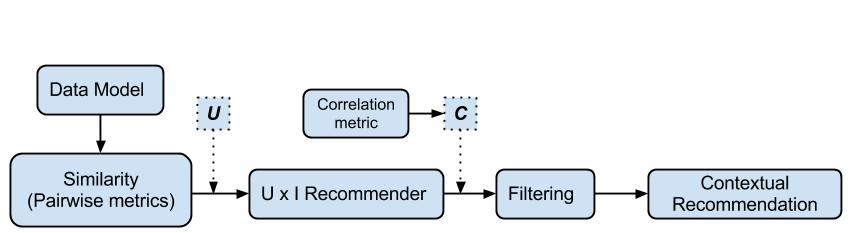
\includegraphics[width=3.5in]{archdiagram.jpg}
\caption{Contextual post-filtering for recommendation systems}
\label{archdiag}
\end{figure}

Figure ~\ref{archdiag} shows the overall architecture of the recommendation system. The \textit{Data Model} represents the pre-processed dataset where the dataset is read from a csv file and stored into two separate data stores corresponding to user and movie attributes respectively. Based on the similarity metric, other users who have given similar ratings to the user under consideration were found out.     The two similarity metrics used were

\begin{itemize}
\item Euclidean distance 
\item Pearson correlation
\end{itemize}


The results from previous step were used in Collaborative Filtering which generates a recommendation of the movies for given user by looking at other users who have similar tastes. These recommendations are then passed through the contextual filtering step, where the results are filtered based on contextual attributes(user-specific or general) computed using different methods. After this step a contextualized result in the form of a ranked list of movie recommendations is obtained. The block \textit{U} represent the active user under consideration for the recommender system and \textit{C} represents the context for the contextual-filtering step. The correlation metric helps refine the context attribute for the filtering approach. The following sections describe in detail each of these steps.

\subsection{Dataset}
We used the LDOS - CoMoDa dataset \cite{kovsir2011database}, made available by Dr. Andrej Kosir from the University of Ljubljana, Slovenia. The LDOS - CoMoDa dataset is a context-rich movie recommender dataset, which contains ratings for movies along with contextual information describing the situations in which the movies were watched. 
It contains 30 variables among which are 12 contextual variables. The attributes can be classified as:
\begin{enumerate}
\item \emph{User Attributes}: ID, Sex, Age, City, Country
\item \emph{Movie Metadata}: rating, director, language, country, genre(s), actor(s), budget
\item \emph{Context attributes}: time,weather, daytype, season, location, social, end emotion, dominant emotion, mood, physical
\end{enumerate}
The value for each non-numerical discrete attribute is represented with a distinct number. The training instances for the recommendation system consists of the user, movie and context attributes for a single user and the corresponding rating associated with it. A single user can have multiple ratings, indicating he has rated more than one movie. The dataset consists of 2296 instances (ratings), with 121 unique users. 

\subsection{Cleaning the data}

The LDOS-CoMoDa dataset was converted into csv format to make it easy for parsing. The dataset is read and stored in pandas dataframe \footnote{http://pandas.pydata.org/} object replacing all the missing values(-1) using the mean of the available values. We maintain two separate dictionaries for user attributes (indexed by the user ID) and movie attributes (indexed by the movie ID). The movie attributes are mapped to individual users by the movie ID, as part of the values associated with each user instance. The structure of these dictionaries are given below.

users = 
	{userid: 
		{itemid:  
			rating, 
			age,
			sex,
			city,
			country, 
			c1,
			.
			.
			c12}}

items = 
	{itemid: 
		{director, 
		a1..a3,
		g1..g3, 
		budget, 
		language, 
		country}}
$c_{i}$ denote contextual attributes.

\subsection{Collaborative Filtering}
In Collaborative Filtering, the recommendations are generated based on a user and her previous movie ratings. First step in the process is to compute the similarity score to estimate users who are most similar to the given user. Higher values of similarity score meant that pair of users under consideration were similar. After finding out the users with similar tastes, we sorted them in descending order so as to obtain a ranked list of similar users. To generate recommendation the items were scored by producing a weighted score that
ranks the users. The movie ratings of the other similar users were multiplied with the similarity score to obtain the weighted score for each unseen movie. These were returned in descending order of the weighted score as recommendation. \cite{segaran2008programming}  

\subsection{Building the User Profile}

A User Profile consists of contextual attributes which are used for contextual filtering of recommendations. The following methods were used for finding out the significant contextual attributes.

\subsubsection{Feature Selection}

The first method was used to find out existence of important contextual features for the entire dataset. These features might help in boosting the performance of recommender systems. Forest of trees were used to evaluate the importance of features in the dataset. Tree-based estimators from the sklearn.tree module and forest of trees in the sklearn.ensemble module were used for the purpose. Univariate chi2 feature selection was also tried for the purpose but didn't give *interpretable* results. 

\subsubsection{Information Gain}

Information gain helps bias the decision making process by considering features that are relevant. Information gain is particularly effective, since the attributes in LDOS-CoMoDa are primarily nominal and take up a finite (small) set of values. The ratings given by each user were considered in isolation for computing the information gain of each attribute. Compared to the first method, this method a tailored set of attributes specific to each user. We built a user profile for every user in the dataset, based on the context attributes with the highest information gain. This calculation was done on the basis of the ratings given for a movie watched by the user, under the context features described for the same.

\subsubsection{Clustering}


\subsection{Contextual filtering}
In this module, we refine the results provided by the Collaborative Filtering system, based on the filtered context features from the previous step. The model generates a recommendation of movies for a particular test user instance. A single test instance is a user profile, for which a third of the total set of movie ratings that were present are removed. The recommendation process starts when the user enters a set of attributes describing his context. These contextual features are compared with the user profile built in the previous step. For every (movie, rating) recommendation pair from collaborative filtering, we check if the rating is higher than an optimum value (For our dataset, we chose 4, since that was the average rating for a "good" movie). If there is a possible match, the (movie, rating) combination is appended to the set of final recommendations to be provided to the user. These recommendations are not only based on the similarity in tastes between users, but also customized for the user based on his context.

\section{Intuition}

\section{Experiments}
Table~\ref{ldos} demonstrates the statistics of the LDOS - CoMoDa dataset. This information and further demographics on the dataset will be calculated. These demographics will help identify the correlation not only between the contextual attributes and the movie's ratings, but also include user profiles. For example, it was observed that when the dominant mood was "Happy", the overall ratings, regardless of the other attributes, were high (ranging from 4 to 5). This sets up a correlation, of the contextual attribute modeling the mood of the user, to be a significant parameter for recommending a movie with higher rating. The number of ratings per user and per item have also been analyzed and are added to the Appendix.

\begin{table} [H]
	\caption{LDOS - CoMoDa dataset statistic}
	\centering        
    \begin{tabular}{l|l}
    \hline
    Number of users            & 121 \\
    Number of items            & 1233  \\
    Number of ratings          & 2294  \\
    Average age                & 28  \\
    Number of countries        & 6  \\
    Number of cities           & 18  \\
    Max ratings of single user & 220  \\
    Min ratings of single user & 1  \\
    \end{tabular}
    \label{ldos}
\end{table}

\subsection{Precision/Recall of Contextual Filtering}
An effective method to evaluate a recommender's suggestions, is to grade the quality of its estimated preference values. This involves measuring how closely the estimated preferences match the actual preferences of the user. In order to evaluate the accuracy of our recommender engine , we use a precision-recall measure where the predicted movie recommendations, and their respective ratings, are compared with the removed ratings. The precision metric finds the proportion of relevant movies from the list of (movie, rating) recommendation pairs. The recall measures the proportion of movies that were recommended from the total list of all possible movies. 

The recommended movies are based on a rating margin of +1 and -1. This flexibility, though can reduce the recall slightly, removes the possibility of no recommendations being generated for a particular user and the provided context.

\subsection{Clustering based on User profiles}
 We experimented on alternative techniques on characterizing 

Attribute      Full Data          0          1          2          3          4
                  (2296)      (267)      (322)      (721)      (596)      (390)
===============================================================================
age               28.418    31.7963    25.6773    29.6492    28.3657    26.1719
sex                 Male     Female       Male       Male     Female       Male
country               UK         UK    Denmark         UK         UK    Denmark
time             Evening      Night    Evening    Evening    Evening      Night
daytype          Weekend    Weekend    Working    Working    Working    Weekend
season            Winter     Autumn     Autumn     Autumn     Winter     Winter
location            Home       Home       Home       Home       Home       Home
weather            Sunny      Rainy      Sunny      Sunny     Cloudy     Cloudy
social             Alone      Alone      Alone    Partner      Alone    Partner
endEmo             Happy    Neutral    Neutral      Happy    Neutral    Neutral
dominantEmo      Neutral    Neutral    Neutral      Happy    Neutral    Neutral
mood            Positive    Neutral    Neutral   Positive    Neutral   Positive
physical         Healthy    Healthy    Healthy    Healthy    Healthy    Healthy
decision        Decision   Decision      Given   Decision   Decision      Given
interaction        First      First      First      First      First      First

Cluster 0 <-- 1
Cluster 1 <-- 2
Cluster 2 <-- 5
Cluster 3 <-- 3
Cluster 4 <-- 4


\subsection{Clustering experiment} 
Give statistics on the clustering - explain how it fared



%\subsection{Implementation}
%  
%
%The closest matches to an user were found out by comparing each user with every user and ranking the similarity scores in descending order. By limiting the number of results thus obtained, a list of top 5 similar users to a specific user can be obtained.
%
%We plan to also user Pearson correlation coefficient as the similarity metric and compare the accuracy of that with Euclidean distance similarity metric. Also by using the weighted average of ratings per user,  recommendations for an user can be obtained. 
%
%Once the simple recommendations system is completed, other attributes will be added into recommendation system for filtering the results. The predictive features that is which of user attributes, movie attributes and context attributes are strongly correlated with labels, will be identified. 


\section{Conclusions}
The CAMR system demonstrates the usage of contextual information as a relevant set of features, when providing recommendations. The system not only incorporates user tastes with similar profiles and ratings, but also filters the recommendations based on the current context of the active user. The recommendations are improved by understanding the correlation metrics between features that affect the outcome of the movie ratings, and thereby altering the filtering approach. Identification of common contextual features among users and their influence on the movie ratings can be analyzed via training on decision trees based on the contextual features. Decision trees modeled for separate user profiles can be used to analyze the relationship of context on the rating as well as the selection of movies for recommendation. This recommender system can be extended to incorporate machine learning techniques such as a support vector machine (SVM). The SVM can help classify the set of liked and disliked items of a user in different contexts as classes and constructs a separating hyperplane which maximizes the separation between them. It also remains to be seen if the contextual attributes affect the movie selection or movie rating or both.


Incorporating such rich set of contextual features helps personalize a recommendation process, and provides value addition to a recommender system.

\section{Appendix}

%\subsection{Plan of activities}
%
%\begin{enumerate}
%\item Identify predictive features from user attributes, movie attributes and context attributes that are strongly correlated with labels
%\item Understand univariate feature selection and use it for feature selection/dimensionality reduction on the data set to improve reccommender's predicted ratings, or to boost their performance on very high-dimensional datasets
%\item Implement post-filtering based on the context attributes selected from previous two steps. 
%\item Comparison of predicted ratings accuracies by filtering based on user, item and context-based attributes. 
%\item Learn to use the python shelve model and try to use persistent data structures for storing the data model so that once it is trained, it can be reused any number of times
%\end{enumerate}
%
%\subsection{Before Midterm}
%\begin{enumerate}
%\item Survey of recommender system techniques such as collaborative filtering, Content-based systems  as well as possibility of using DBpedia to boost  the quality of recommendations\cite{ostuni2012cinemappy} and postfiltering of data based on various contextual information
%\item Selection of tools and libraries to be used such as scikits learn, pandas, statsmodes and pylab.
%\item Reading and storing the data in a data model for analysis as well as computations.
%\item Identifying important features by measuring correlation among features and possibly visualize to identify positive and negative correlations
%\item Use chi-square feature selection for  selecting predictive features.
%\end{enumerate}

\subsection{Dataset Analysis}

\begin{figure}[H]
\centering
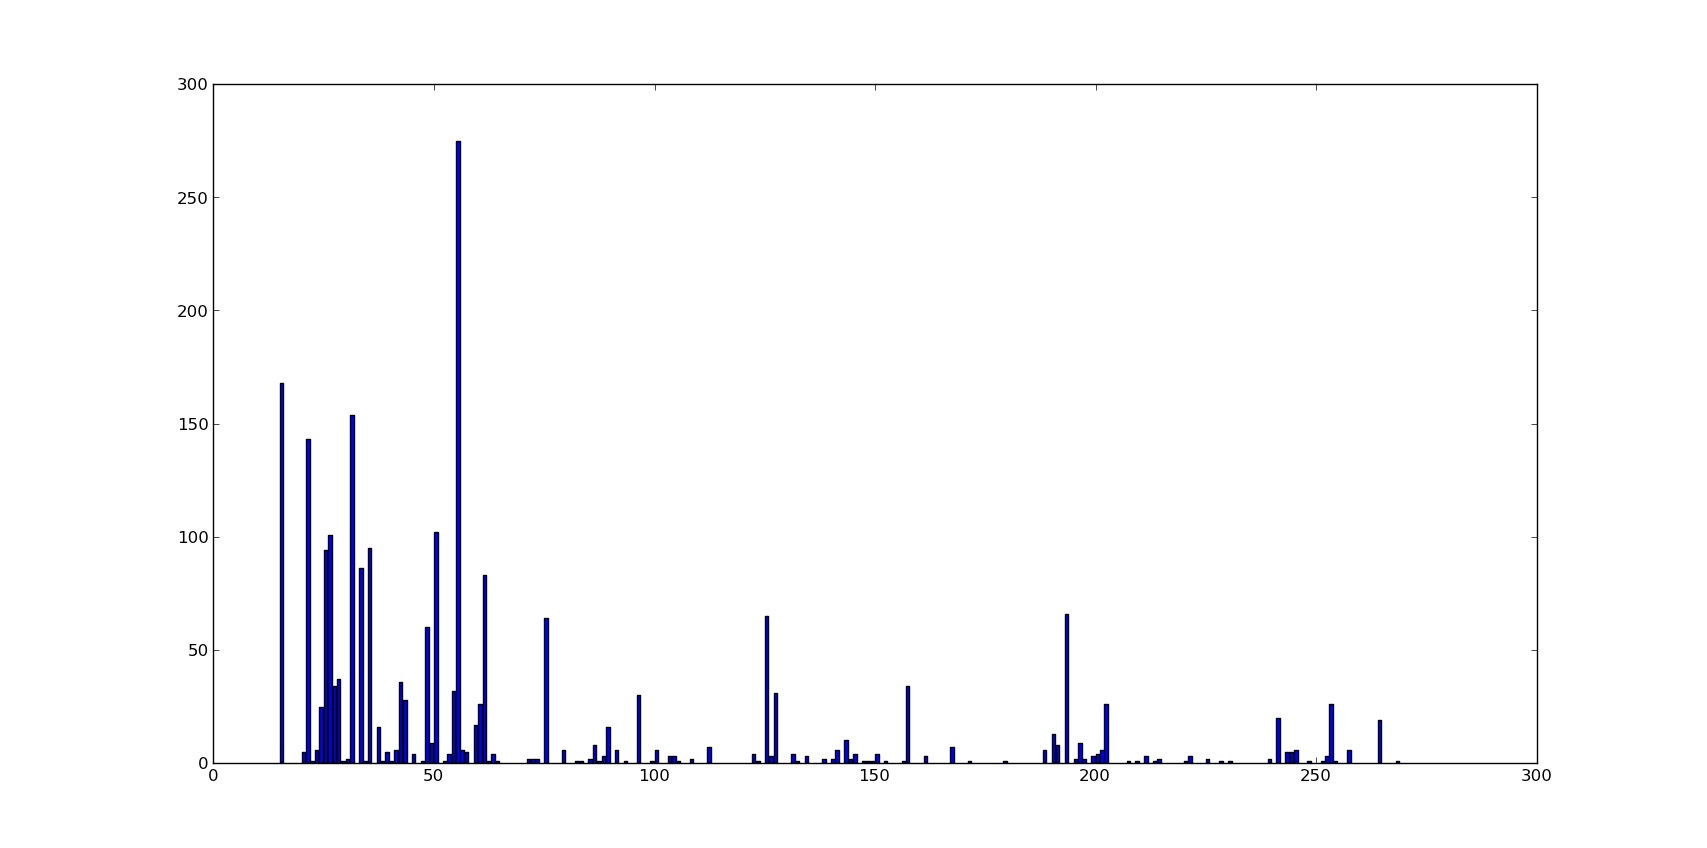
\includegraphics[height=2.5in, width=4in]{ratingsperuser.png}
\caption{Ratings per user}
\label{ruser}
\end{figure}

\begin{figure}[H]
\centering
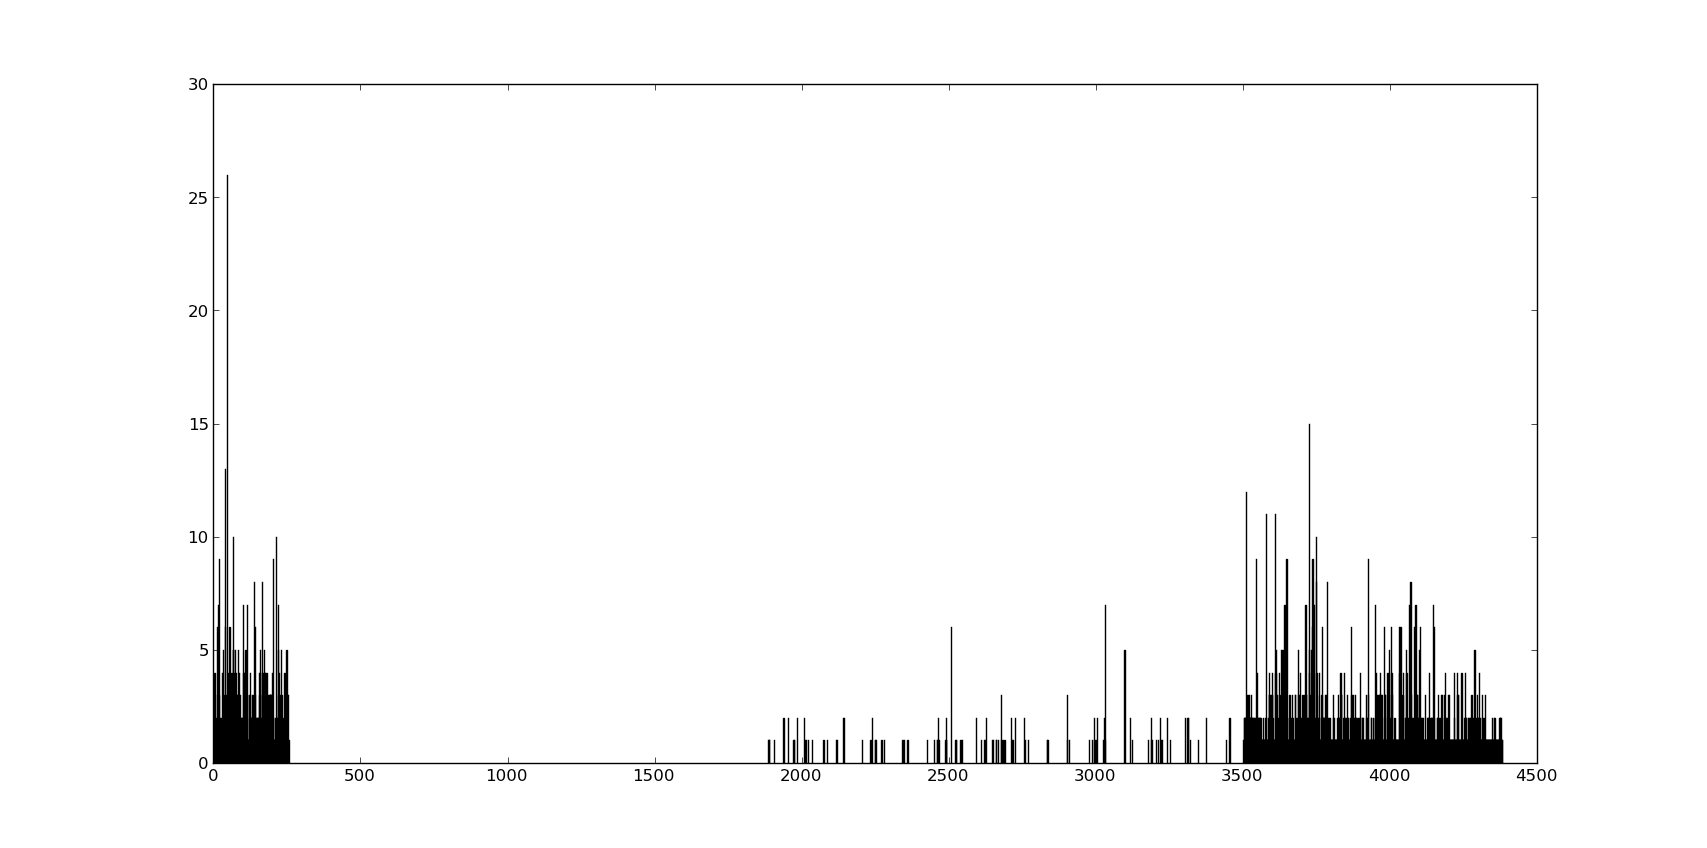
\includegraphics[height=2.5in, width=4in]{ratungspermovie.png}
\caption{Ratings per item}
\label{ritem}
\end{figure}

\bibliography{pr_ref}
\bibliographystyle{icml2011}

\end{document}
